\section{Results}
\label{sec:results}

\subsection{Area measurements}
Area measurements obtained using color blob detection/segmentation in \Matlab\ are shown in \fref{tab:results:area}.
\begin{table}[h]
\caption{Area normal to flow for \Cxparadisi\ specimen and rigid physical model of a single grapefruit leaf.}
\label{tab:results:area}
\begin{center}
\begin{tabular}{cc}
\toprule
& area, \si{\meter\squared} \\
\midrule
\Cxparadisi\ grapefruit specimen & 0.223 \\
rigid physical model of leaf (metal) & 0.0346 \\
\bottomrule
\end{tabular}
\end{center}
\end{table}






\subsection{Drag measurements}
\Fref{tab:results:displacement} gives the measured raw displacement data for the \Cxparadisi\ specimen and the rigid physical model of a single grapefruit leaf. The resulting drag estimates are summarized in \fref{tab:results:drag} and figures~\ref{fig:results:drag} and \ref{fig:results:dragarea}. \Fref{fig:results:drag} shows the drag results; the magnitude of the drag force is smaller for the much smaller metal leaf (two-way ANOVA, $p<\num{4.6e-10}$, $n=5$). However, when the drag is normalized by area, the effect of leaf flexibility becomes apparent. \Fref{fig:results:dragarea} shows the drag/area ratio increases with fan speed (two-way ANOVA, $p=0.025$, $n=5$) and shows that the mean drag on the metal, rigid physical model of a single leaf is 19\% higher than for the \Cxparadisi\ specimen at the same speed, though the latter effect is not statistically significant (two-way ANOVA, $p=0.3207$) due to measurement error and the low number of samples ($n=5$).
\clearpage 
\begin{table}
\caption{Measured raw displacement (\SI{e-3}{\meter}) for \Cxparadisi\ grapefruit specimen and rigid physical model of a single leaf (metal).}
\label{tab:results:displacement}
\begin{center}
\begin{tabular}{cccc}
\toprule
grapefruit & grapefruit & grapefruit & metal leaf \\
speed 1 & speed 2 & speed 3 & speed 3 \\ 
\midrule
%0.156 & 0.250 & 0.313 & 0.200 \\ % inches / cm 
%0.188 & 0.188 & 0.250 & 0.0500 \\
%0.250 & 0.250 & 0.313 & 0.100 \\
%0.188 & 0.219 & 0.313 & 0.200 \\
%0.188 & 0.250 & 0.313 & 0.150 \\
3.97 & 6.35 & 7.94 & 2.00 \\ % convert all to SI units these are 10^3 m
4.76 & 4.76 & 6.35 & 0.50 \\
6.35 & 6.35 & 7.94 & 1.00 \\
4.76 & 5.56 & 7.94 & 2.00 \\
4.76 & 6.35 & 7.94 & 1.50 \\
\bottomrule
\end{tabular}
\end{center}
\end{table}
\begin{table}
\caption{Summary of drag estimates (mean$\pm$s.d.) for \Cxparadisi\ grapefruit specimen and rigid physical model of a single leaf (metal).}
\label{tab:results:drag}
\begin{center}
%\begin{tabular}{lcccc} % table as wide format for slides
%\toprule
%& grapefruit & grapefruit & grapefruit & metal leaf \\
%& speed 1 & speed 2 & speed 3 & speed 3 \\
%\midrule
%drag, \si{\newton} & \num{0.051\pm0.008} & \num{0.061\pm0.007} & \num{0.079\pm0.007} & \num{0.014\pm0.007} \\
%drag/area, \si{\newton\per\meter\squared} & \num{2.4\pm0.4} & \num{2.9\pm0.3} & \num{3.7\pm0.3} & \num{4.5\pm2.1} \\
%\bottomrule
%\end{tabular}
\begin{tabular}{lcc} % table as narrow format for journal
\toprule
& drag & drag/area \\
& \si{\newton} & \si{\newton\per\meter\squared} \\
\midrule
grapefruit, speed 1 & \num{0.051\pm0.008} & \num{2.4\pm0.4} \\
grapefruit, speed 2 & \num{0.061\pm0.007} & \num{2.9\pm0.3} \\
grapefruit, speed 3 & \num{0.079\pm0.007} & \num{3.7\pm0.3} \\
metal leaf, speed 3 & \num{0.014\pm0.007} & \num{4.5\pm2.1} \\
\bottomrule
\end{tabular}
\end{center}
\end{table}

\clearpage
\begin{figure}[p]
\begin{center}
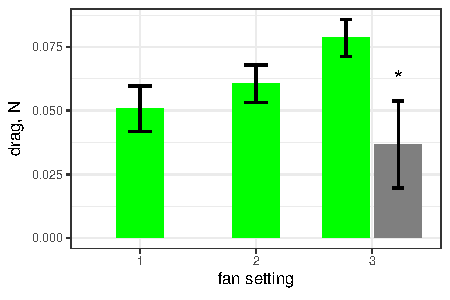
\includegraphics{data/results1.pdf}
%\includesvg{data/results1}
\end{center}
\caption{Drag (mean$\pm$s.d.) for \Cxparadisi\ grapefruit specimen (green) and metal rigid physical model (gray) at different fan speeds. The rigid physical model leaf has less drag than the intact \Cxparadisi\ specimen because of smaller area (two-way ANOVA, $p<\num{4.6e-10}$, $n=5$).}
\label{fig:results:drag}
\end{figure}

\begin{figure}[p]
\begin{center}
\includegraphics{data/results2.pdf}
%\includesvg{data/results2}
\end{center}
\caption{Drag, normalized by area, (mean$\pm$s.d.) for \Cxparadisi\ grapefruit specimen (green) and metal rigid physical model (gray) leaves at different fan speeds. Normalized by area, the rigid metal leaf experiences 19\% more drag than the flexible grapefruit leaves at the same speed, however, the differences are not statistically significant consider the small number of replicates and measurement noise (two-way ANOVA, $p=0.3207$, $n=5$). Differences in drag on the \Cxparadisi\ specimen are statistically significant at different speeds ($p=0.025$, $n=5$).}
\label{fig:results:dragarea}
\end{figure}

\clearpage
\begin{figure}
\begin{center}
%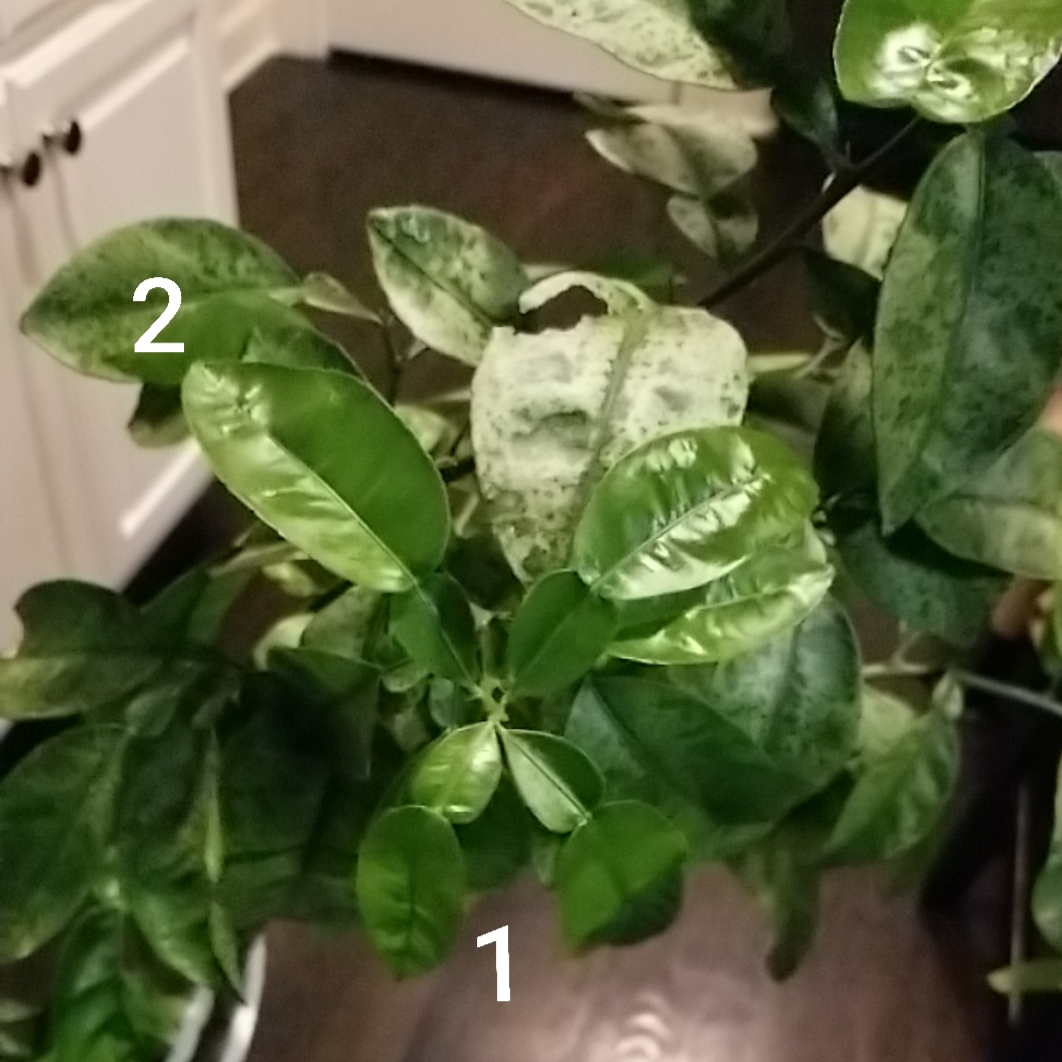
\includegraphics[width=0.49\columnwidth]{figures/Snapshot1.jpg}
%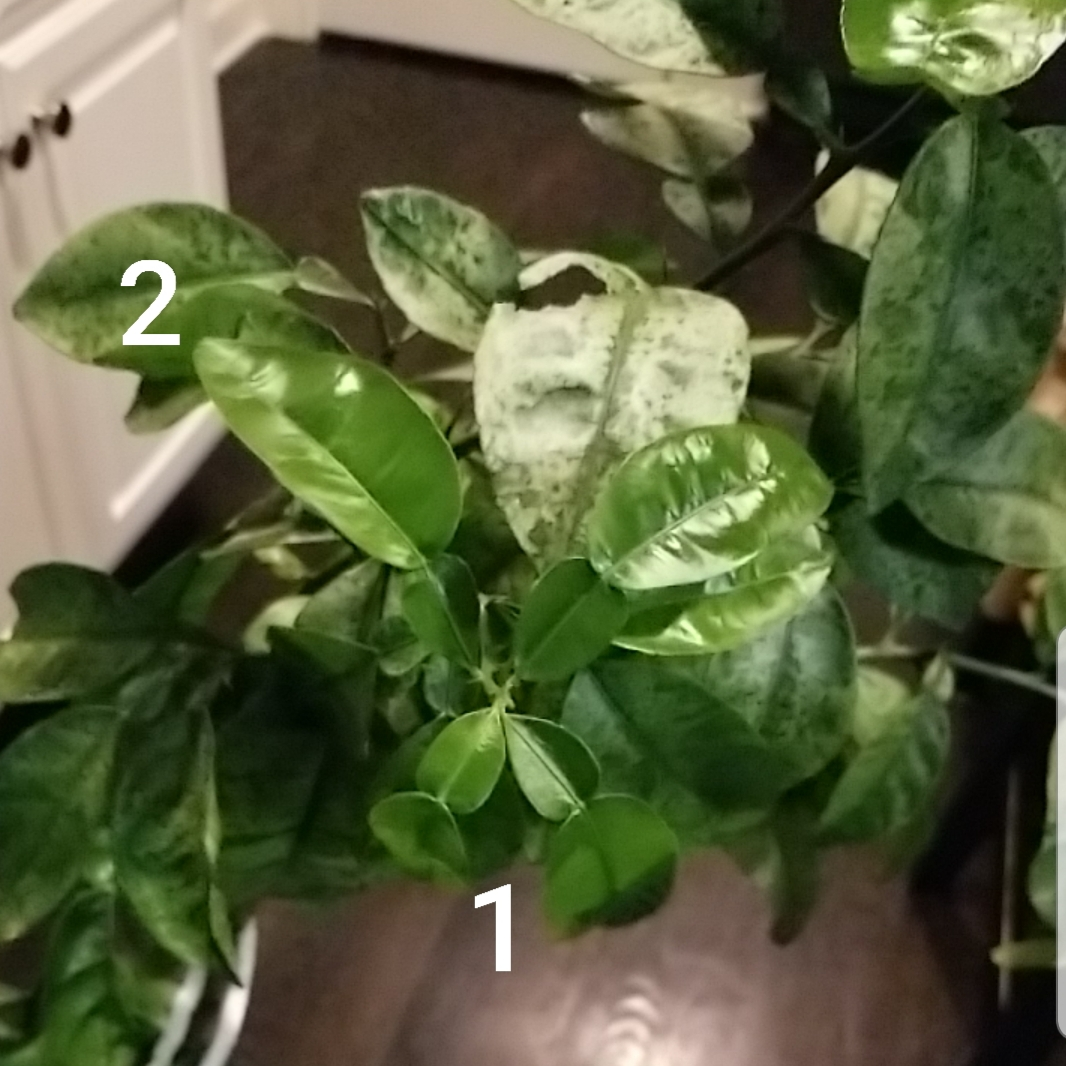
\includegraphics[width=0.49\columnwidth]{figures/Snapshot2.jpg}\\
%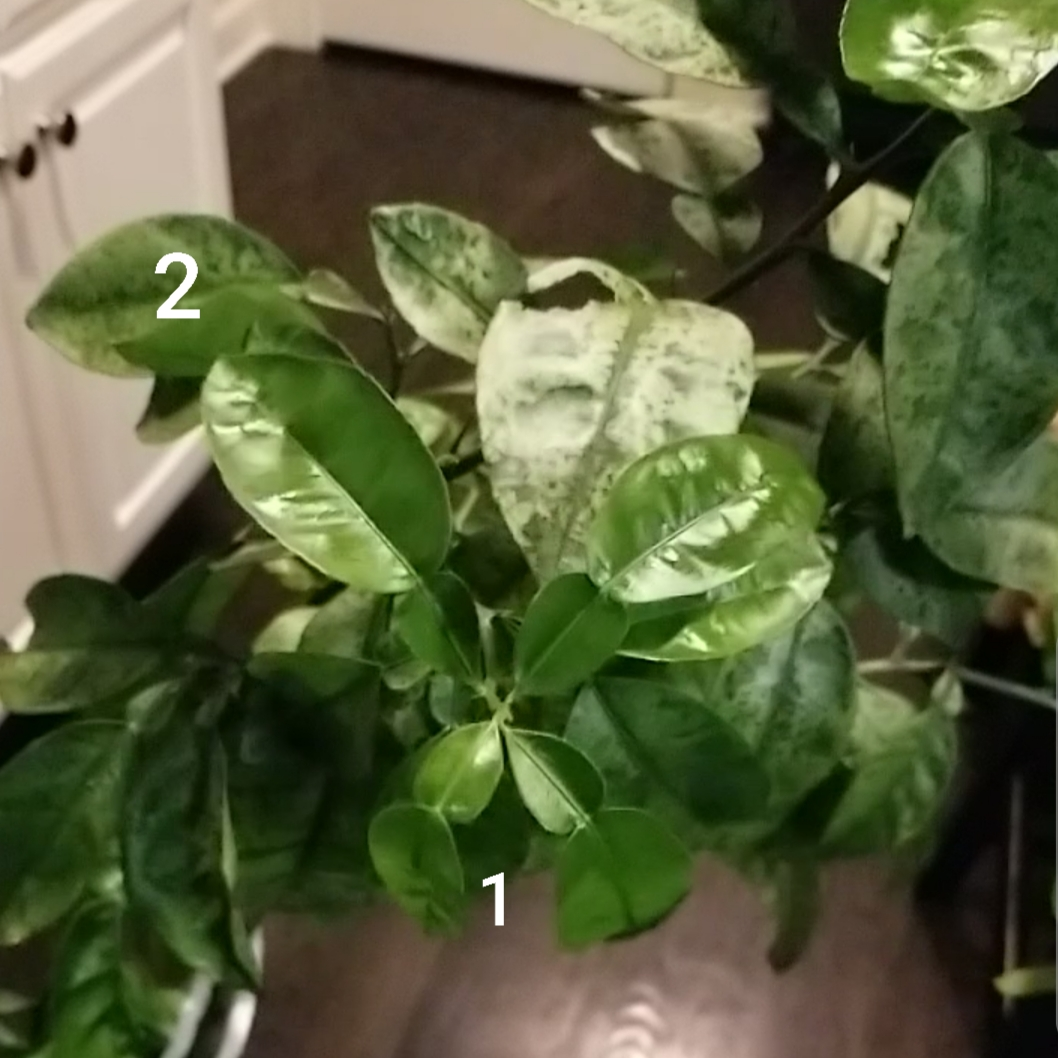
\includegraphics[width=0.49\columnwidth]{figures/Snapshot3.jpg}
%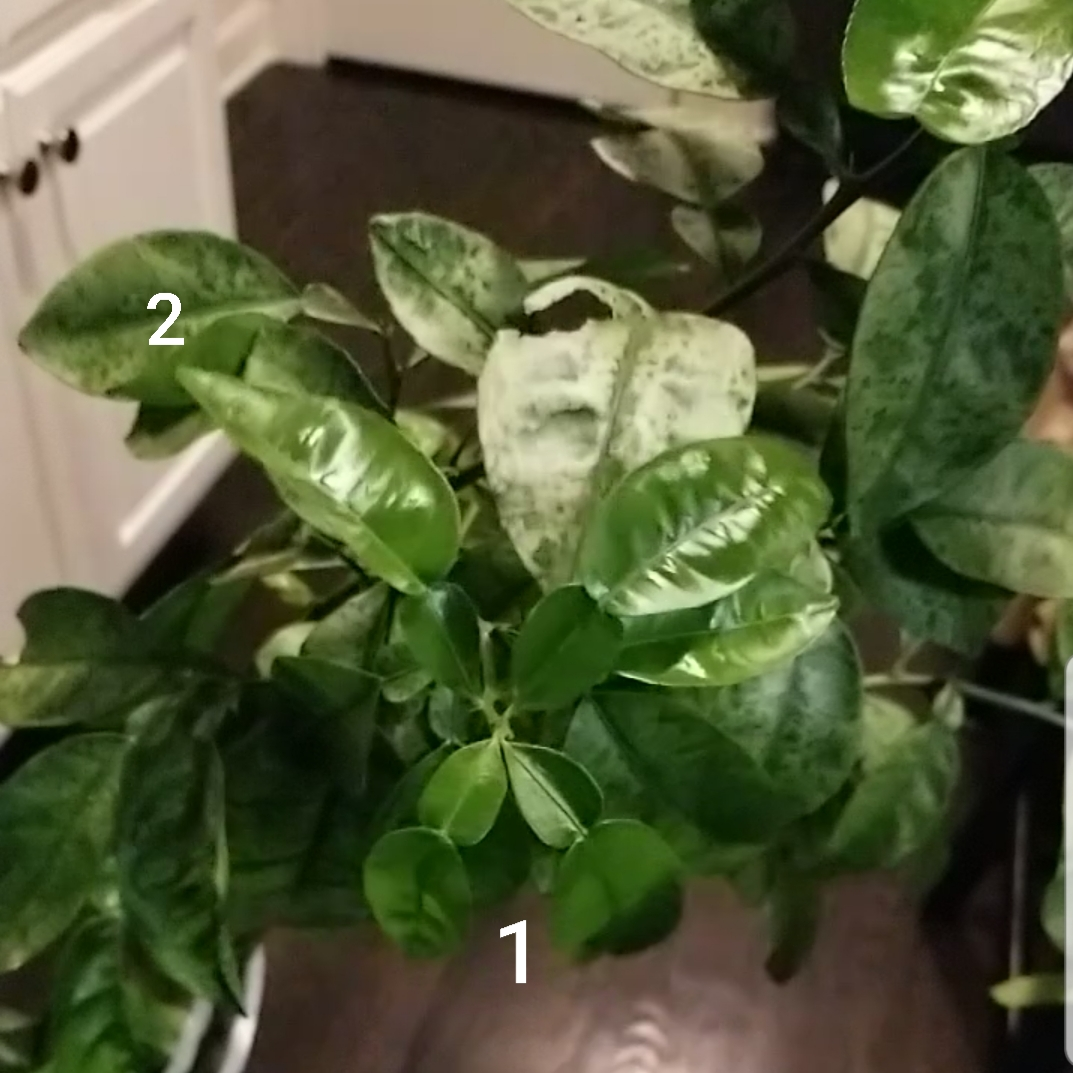
\includegraphics[width=0.49\columnwidth]{figures/Snapshot4.jpg}
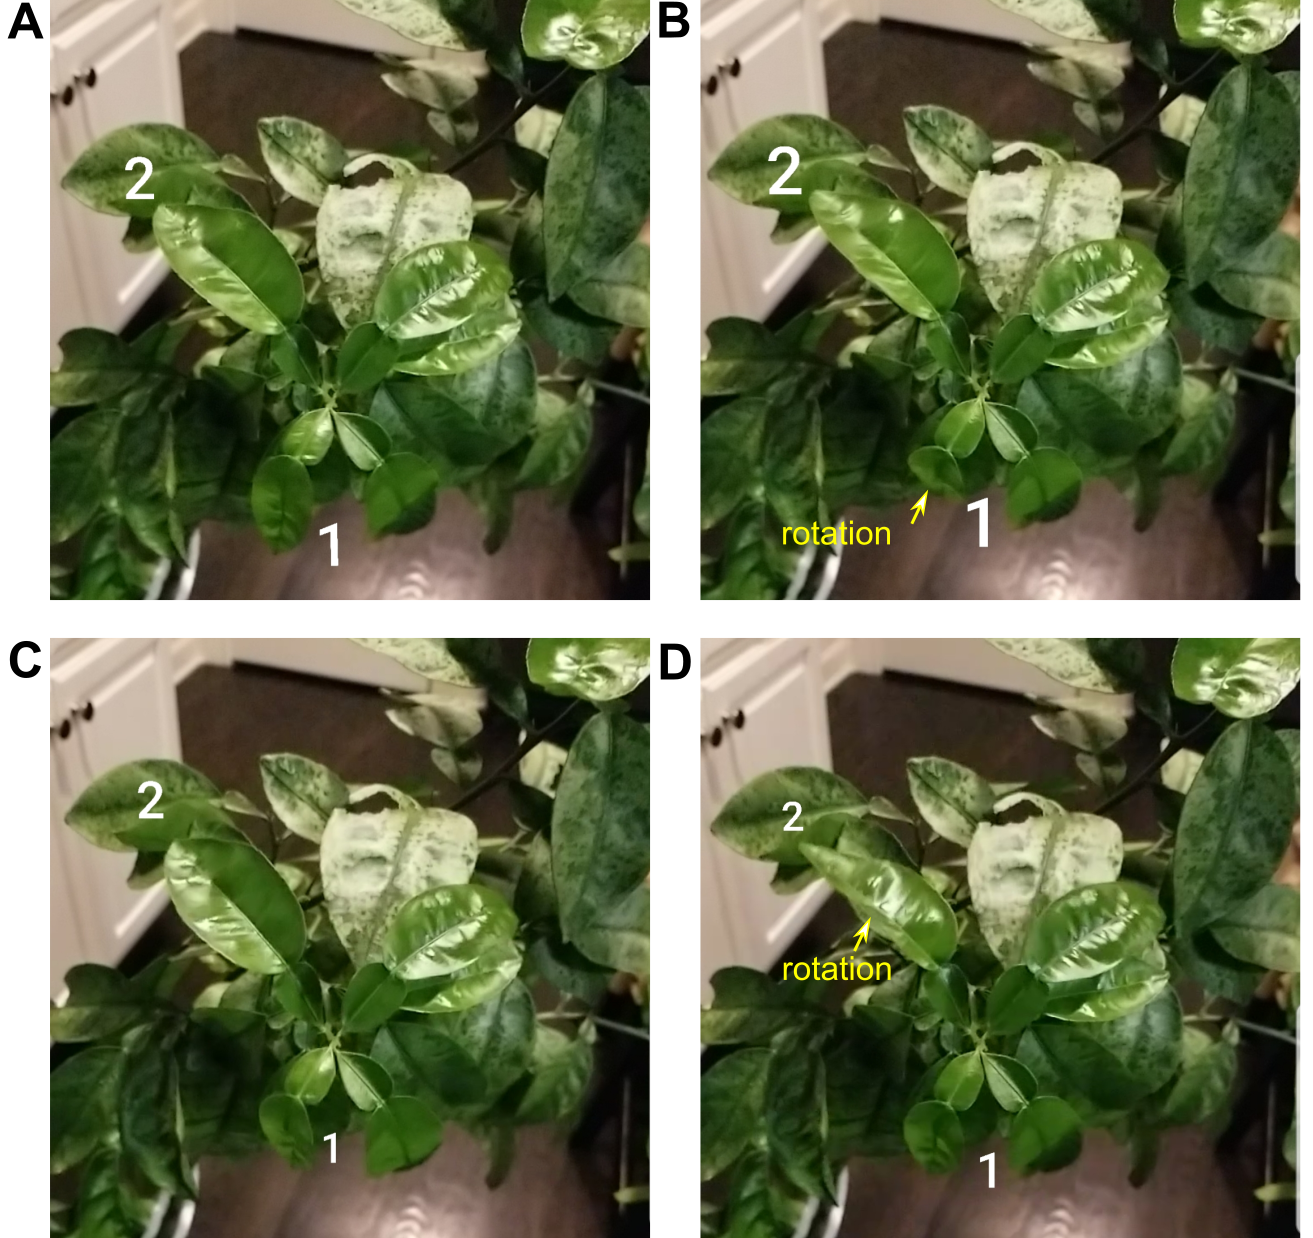
\includegraphics{figures/fig6.png}
\end{center}
\caption{Example frames from slow motion video of \Cxparadisi\ specimen at fan speed 3. Leaves marked 1 (A, B) and 2 (C, D) rotate at the petiole, reducing by half their area normal to the flow. Images are \SIrange{4}{13}{\milli\second} apart.}
\label{fig:results:leafmovement}
\end{figure}





\subsection{Leaf movement during flow}
% This bit needs some help. 
\Fref{fig:results:leafmovement} shows frames from the slow motion video of \Cxparadisi\ at fan speed 3. Following the leaves indicated by the number 1, the leaves which were struck head-on by the wind flexed quite far at their joints, exposing roughly half of their surface area to the camera. The leaf indicated with the number 2 in \fref{fig:results:leafmovement} also pivoted at its joint, and exposed about half of its area to the wind before returning to its previous state. The process is dynamic, with leaves feathering and returning to their neutral position in approximately three video frames, or \SI{13}{\milli\second}. 

